\newpage
\fancyhead[C]{Jihwan Shin}
\section{Mission Planning} \label{sec:missionplanning}

%%%%%%%%%%
\subsection{Introduction}
\label{sec:msp_introduction}

\subsubsection{Objectives}

The mission planning of the multi-aerial drone system focuses on how to efficiently plan the paths of the drones to fully survey our \gls{roi} using the chosen suite of sensors. The input will be the user-defined \gls{roi} and the specifications of the drone dynamics and sensors, which go through the mission planning algorithm to output the set of coordinates each drone must follow (Figure~\ref{fig:msp_objective}).

\begin{figure}[h]
    \centering
    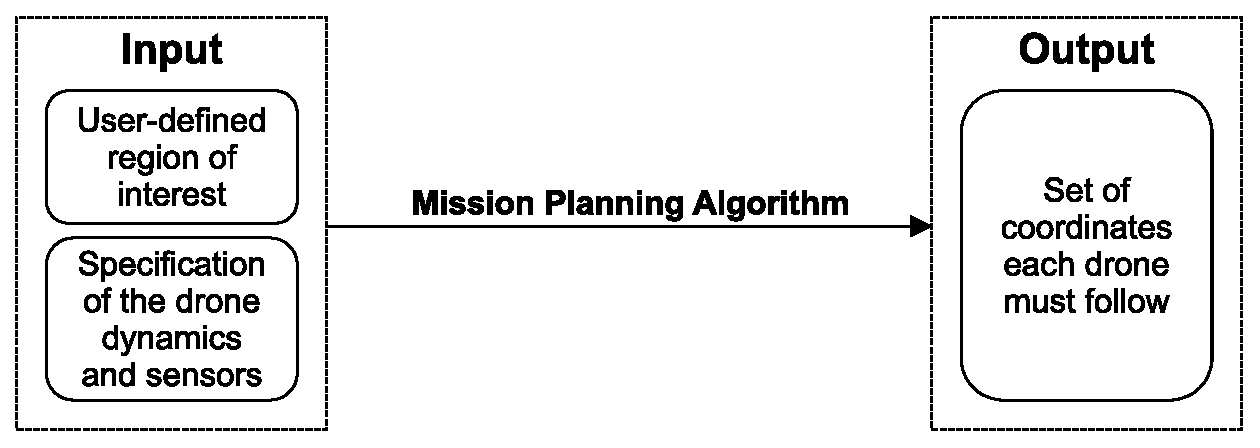
\includegraphics[width=0.7\linewidth]{figs/Jihwan/Objective of the Mission Planning System.eps}
    \caption[Objective of the Mission Planning System]
    {Objective of the mission planning system.}
    \label{fig:msp_objective}
\end{figure}

To have a successful mission planning framework, we wish to meet the following criteria:

\begin{itemize}
    \item \textbf{Efficient}: The system should be efficient in terms of time, resource and costs compared to the previous manual demining methods. 
    \item \textbf{Expandable}: The system should be expandable to a larger area of land by adding additional drones and base stations as necessary. 
    \item \textbf{Intuitive}: The system should be easily usable by the members of demining organisations even without professional software knowledge. 
\end{itemize}

This section will explain the theoretical basis of how the mission planning algorithm works, then demonstrate how it meets the criteria above through a real location example. 

\subsubsection{Existing Works}

Existing works focus 

We aim to improve on these works by proposing the \textit{Layered Approach} to the mission planning of our drone system to meet the criterion on efficiency. 

%%%%%%%%%%
\subsection{Layered Approach}
\label{sec:msp_layered_approach}

\subsubsection{Algorithm Outline}

As mentioned in sections~X~and~X, we utilise thermal and \gls{gpr} sensors to detect the landmines. Table~\ref{tab:thermal_vs_gpr} illustrates the trade-off between thermal and \gls{gpr} sensors: a thermal sensor is able to scan at a higher altitude and fast speed which results in a shorter time to survey the given \gls{roi}, but a \gls{gpr} sensor results in a higher confidence in the mine location. 

\begin{table}
    \centering
    \begin{tabular}{|| c || c | c ||}
        \hline
        Sensor & Thermal & \gls{gpr} \\
        \hline\hline
        Altitude & \textbf{High} & Low \\
        \hline
        Speed & \textbf{Fast} & Slow \\
        \hline
        Confidence & Low & \textbf{High} \\
        \hline
    \end{tabular}
    \caption[Comparison of Thermal and \gls{gpr} Sensors]
    {Comparison of thermal and \gls{gpr} sensors. Bold entries indicate an advantage compared to the other sensor.}
    \label{tab:thermal_vs_gpr}
\end{table}

The layered approach aims to optimise between this trade-off by structuring the mission planning algorithm into 6 steps: \textbf{Define}, \textbf{Cover}, \textbf{Analyse}, \textbf{Target}, \textbf{Confirm} and \textbf{Demine}. 

\begin{enumerate}
    \item \textbf{Define}: The \gls{roi} and its obstacles are defined using a \gls{gis} software by the system operator (Section~X).
    \item \textbf{Cover}: The \gls{roi} is fully covered by the thermal sensor in a Boustrophedon (back-and-forth) path through a \gls{cpp} algorithm (Section~X).
    \item \textbf{Analyse}: The resulting thermal sensor readings are analysed by a machine learning algorithm to return a list of suspected landmine points (Section~X). 
    \item \textbf{Target}: The suspected landmine points are targeted and rescanned by the \gls{gpr} sensor in a minimum traversal path through a \gls{tspo} algorithm (Section~X). 
    \item \textbf{Confirm}: The resulting \gls{gpr} readings are analysed by a machine learning algorithm to return the final result on the locations of the landmines (Section~X). 
    \item \textbf{Demine}: The \gls{roi} is demined based on the generated landmine location map. The demining operation itself is outside the scope of this project, and it will be the responsibility of the demining organisations to safely deactivate and remove the mines.
\end{enumerate}

%%%%%%%%%%
\subsection{Defining the Region of Interest}
\label{sec:msp_define}

\subsubsection{Geometric Representation}

The \gls{roi} is an abstract representation of the minefield we wish to survey using our multi-aerial drone system. To apply geometric operations as required by the mission planning algorithm, we represent the \gls{roi} as a Polygon with Holes class (\texttt{Polygon\_with\_holes\_2}) from the \gls{cgal}\footnote{\url{https://www.cgal.org/}} which defines the outer boundary and its holes (obstacles) as a set of vertex coordinates \cite{cgal2024pwh}. \gls{cgal} provides various algorithms that can be directly applied to a Polygon with Holes object -- some of them will be explored and applied in later sections of this report to construct the mission planning algorithm. 

\subsubsection{Geographic Information System}

\gls{gis} software connects the geometric representation of the \gls{roi} to a geographic map in an accessible user-interface. This project uses a free and open-source \gls{gis} software called \gls{qgis}\footnote{\url{https://qgis.org/}} from which the demining operator can define the \gls{roi}. The process of defining the \gls{roi} on \gls{qgis} is shown in Figure~\ref{fig:msp_qgis}. Once all the outer polygon and its holes have been created to define the full \gls{roi}, the operator can export the coordinates in a GeoJSON\footnote{\url{https://geojson.org/}} format which gets converted into a Polygon with Holes object.

\begin{figure}[h]
    \centering
    \begin{tabular}{cc}
        \includegraphics[width=0.45\textwidth]{figs/Jihwan/qgis_a.png} &
        \includegraphics[width=0.45\textwidth]{figs/Jihwan/qgis_b.png} \\
        (a) & (b) \\[10pt]
        \includegraphics[width=0.45\textwidth]{figs/Jihwan/qgis_c.png} &
        \includegraphics[width=0.45\textwidth]{figs/Jihwan/qgis_d.png} \\
        (c) & (d)
    \end{tabular}
    \caption[Demonstration of \gls{roi} Definition using \gls{qgis}]
    {Demonstration of defining the \gls{roi} using \gls{qgis}. \\
    (a) New Shapefile layer is created. \\
    (b) New polygon feature named "Outer Polygon" is defined. \\
    (c) The system operator marks the vertices of the polygon. \\
    (d) The final polygon is displayed. Additional polygons can be added to define the full \gls{roi}.}
    \label{fig:msp_qgis}
\end{figure}

% add note on coordinate system? qgis uses epsg:3857 but it can be changed. 

\subsubsection{Boundary Offset}

In some cases, it may be necessary to ensure that the drones do not exit the \gls{roi} or approach any of its internal obstacles. To do so, a boundary offset can be introduced using the straight skeleton algorithm as suggested in \cite{shahid2024cpp}. The straight skeleton of a polygon can be found by a shrinking process in which the boundary is contracted towards the interior in a self-parallel manner and at the same speed for all edges \cite{aichholzer1996ss}. Applying the shrinking process by a specified length would result in an internal boundary offset of the original polygon. \gls{cgal} provides an implementation for the straight skeleton algorithm which can be directly applied to a Polygon with Holes object \cite{cgal2024ss}.

Figure~\ref{fig:msp_straight_skeleton} shows the result of applying \gls{cgal}'s straight skeleton algorithm to obtain the offset of the \gls{roi} boundary. It shows a successful generation of the boundary offset even for complex geometries, validating this approach for the use case. Furthermore, the size of the offset can be varied depending on the requirements of the mission. The example \gls{roi} was taken from \cite{bahnemann2021cpp} based on a dataset by \cite{sun2014dataset}. 

\begin{figure}[h]
    \centering
    \includegraphics[width=0.7\linewidth]{figs/Jihwan/Polygon Offset with Straight Skeleton.pdf}
    \caption[Boundary Offset of \gls{roi} using Straight Skeleton]
    {The boundary offset of a Polygon with Holes has been generated using \gls{cgal}'s straight skeleton method.}
    \label{fig:msp_straight_skeleton}
\end{figure}

%%%%%%%%%%
\subsection{Coverage Path Planning}
\label{sec:msp_cpp}

\gls{cpp} is a task in which an agent (drone) must cover every point in the given environment (\gls{roi}) with its method of action (thermal sensor reading). To obtain the solution of a \gls{cpp} problem, the \gls{roi} is first decomposed into smaller polygons. In large, this can be distinguished between \textit{approximate} and \textit{exact} cellular decompositions. In an approximate cellular decomposition the \gls{roi} is decomposed into a grid of same size and shape (often a square). Assuming that a single grid is smaller than the size of the sensor's field of view, visiting all grids would indicate a full coverage of the \gls{roi} except the areas which are lost during the approximation process. In contrast, an exact cellular decomposition divides the \gls{roi} into a set of non-intersecting cells which are covered by a continuous path of motion, covering the entire \gls{roi} without missing regions \cite{choset2001surveycpp}. 

For the purpose of a landmine detection system, it is important to use the exact cellular decomposition. This would ensure that no landmines that could cause a safety hazard for the demining individuals have been missed out. In particular, this project uses the boustrophedon cellular decomposition and path planning method that has been implemented by \cite{bahnemann2021cpp} which will be explained in detail below.  

\subsubsection{Boustrophedon Cellular Decomposition and Path Planning}

The boustrophedon cellular decomposition is an exact cellular decomposition method first proposed by \cite{choset1998bcd}. 

\subsubsection{Implementation}

Write here. 

\cite{bahnemann2021cpp}. \ref{fig:msp_bahnemann}.

\begin{figure}[h]
    \centering
    \begin{tabular}{ccc}
        \includegraphics[width=0.3\textwidth]{figs/Jihwan/bahnemann1.png} &
        \includegraphics[width=0.3\textwidth]{figs/Jihwan/bahnemann2.png} &
        \includegraphics[width=0.3\textwidth]{figs/Jihwan/bahnemann3.png} \\
        (a) Input Polygon with Holes & (b) Cell decomposition & (c) Optimal sweep pattern
    \end{tabular}
    \caption[Example of \gls{cpp} by \cite{bahnemann2021cpp}]
    {Example of \gls{cpp} by \cite{bahnemann2021cpp}.}
    \label{fig:msp_bahnemann}
\end{figure}

- talk about how it's written with ros noetic. considerations on porting to ros2 in future versions. using a virutal machine with ubuntu20.04 to run. work pipeline between base computer and virtual machine. 

%%%%%%%%%%
\subsection{Travelling Salesman Problem with Obstacles}
\label{sec:msp_tspo}

\subsubsection{Travelling Salesman Problem}

A \gls{tsp} is an optimisation problem in which the minimum traversal path to visit all targeted nodes in a weighted graph must be found. A number of exact and heuristic solutions have been studied and proposed as reviewed in \cite{laporte1992tsp}. 

- give some examples of exact and heuristic solutions. delve deeper into the heuristic solution that is being used in this report. 

The \gls{tsp} can be extended to more specific cases depending on the application, one of which is the \gls{tspo}. It introduces obstacles which the traversal path must avoid; this is exactly the problem that must be solved for the Target step of the layered approach, as the drone with a \gls{gpr} sensor must visit all suspected landmine points in the obstacle-filled \gls{roi}.

- cite papers which research tspo and list some of the solutions they use. connect to the next section in which we introduce a method for converting tspo into tsp to use a heuristic tsp solution above. 

\subsubsection{Solving TSP-O using Visibility Graph}



Algorithm~\ref{alg:msp_tspo2visgraph}. Figure~\ref{fig:msp_tspo}.

\begin{algorithm}
\caption{Creating the Visibility Graph of \gls{tspo}}
\label{alg:msp_tspo2visgraph}
\begin{algorithmic}[1]
\Require Polygon with Holes $P$, Set of target points $T = \{t_1, t_2, \ldots, t_n\}$ within $P$
\Ensure Visibility graph $G = (V, E)$

\State Initialize visibility graph $G = (V, E)$ with $V = \emptyset$ and $E = \emptyset$
\State $V \leftarrow T$ \Comment{Add all target points to the graph}
\State $V \leftarrow V \cup \text{Vertices}(P)$ \Comment{Add all vertices of polygon with holes to the graph}

\ForAll{$u \in V$}
    \ForAll{$v \in V$ where $u \neq v$}
        \If{$\text{IsVisible}(u, v)$}
            \State $E \leftarrow E \cup \{(u, v, d(u, v))\}$ \Comment{Add edge with Euclidean distance weight}
        \EndIf
    \EndFor
\EndFor

\Return $G$ \Comment{Return visibility graph}
\end{algorithmic}
\end{algorithm}

\begin{figure}[h]
    \centering
    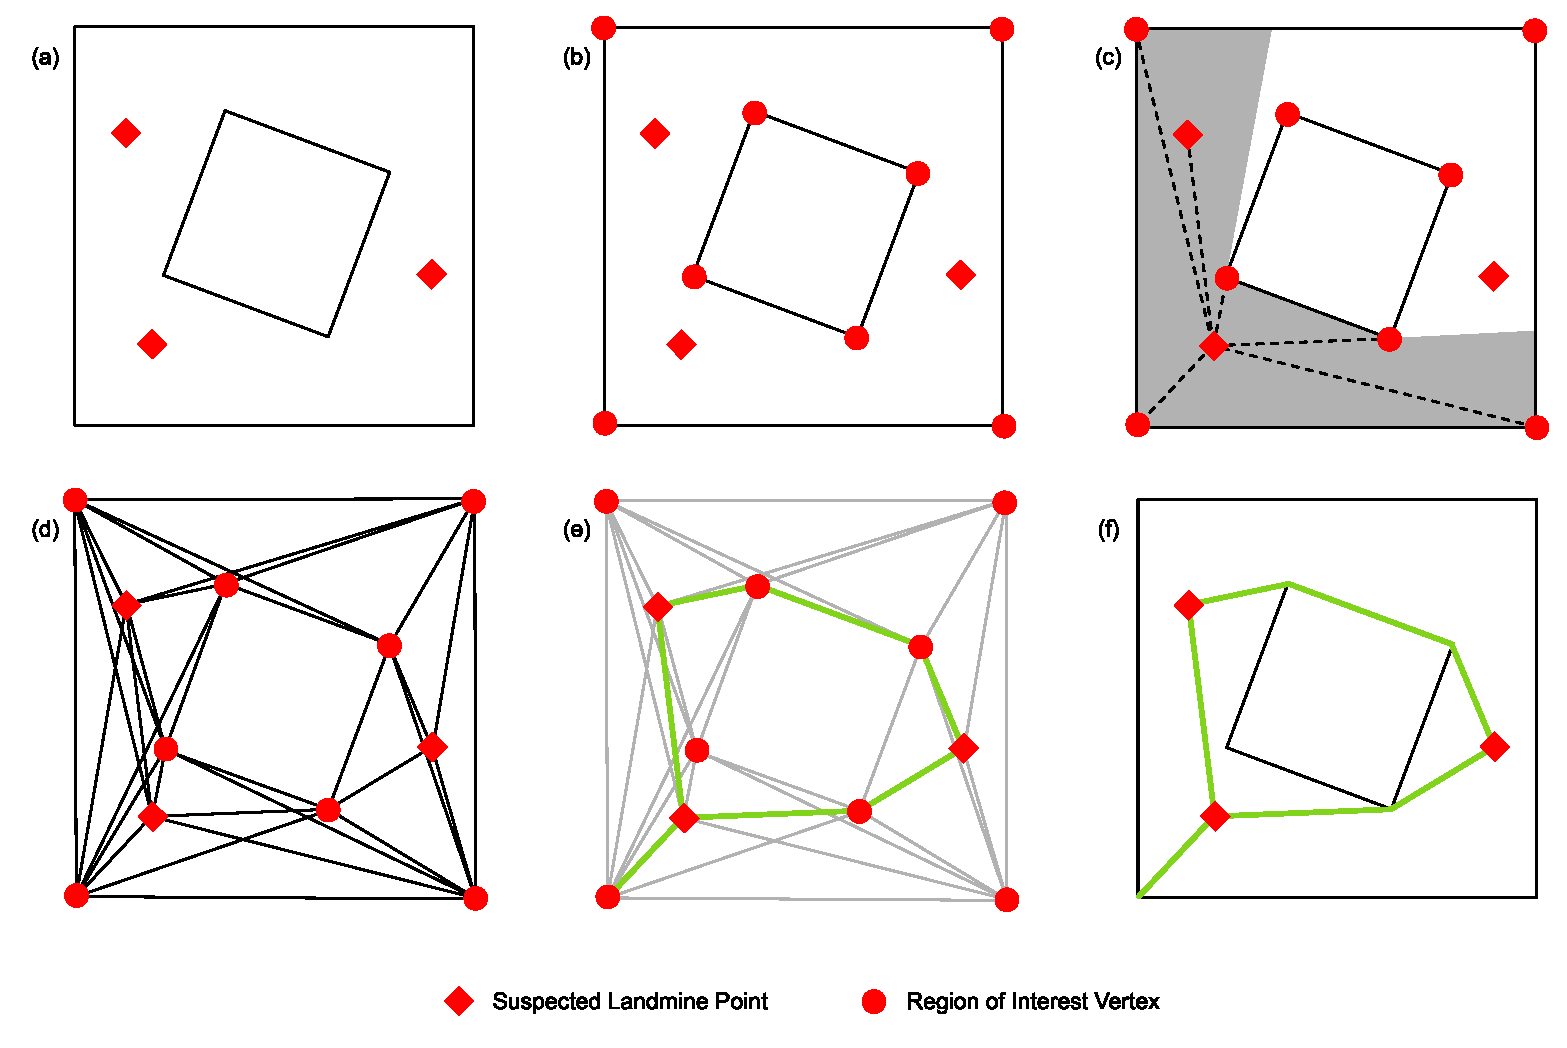
\includegraphics[width=\linewidth]{figs/Jihwan/TSPO Algorithm Visualisation.eps}
    \caption[\gls{tspo} Algorithm Visualisation]
    {\gls{tspo} algorithm visualisation. \\
    (a) The example \gls{roi} is defined to have an outer boundary (outer square) with an obstacle (rotated inner square). Assume three suspected landmine points have been found from the Analyse step. \\
    (b) Add all suspected landmine points and \gls{roi} vertices as nodes to the visibility graph. \\
    (c) For each node, examine which other nodes are visible (i.e. straight line segment between the two nodes is not obstructed by any obstacles). Grey area indicates the visible region of the lower-left suspected landmine point. \\ 
    (d) Add weighted edges between visible nodes, with the weight being the Euclidean distance between them. The figure shows all connected edges between all nodes. \\
    (e) Perform a \gls{tsp} algorithm to visit all suspected landmine points in the visibility graph, starting from and ending at the base station. In this example, the lower left vertex of the outer boundary is defined as the base station. \\
    (f) Final solution of the minimal traversal path to visit all suspected landmine points is displayed, solving the \gls{tspo} algorithm. 
    }
    \label{fig:msp_tspo}
\end{figure}

\subsubsection{Algorithm Complexity}

- big o notation
- give benchmarking with the dataset. x axis on number of points. y axis on number of holes. z axis (colour) on time taken to compute. 

%%%%%%%%%%
\subsection{Expanding to a Multi-Drone Operation}
\label{sec:msp_multi_drone}

Thus far, the mission planning algorithm has been explored for a single-drone operation. To make the system expandable, we must consider how to deploy a multi-drone system using the mission planning algorithm explained above. 

- talk about how a multidrone would involve splitting the region into smaller regions which a single drone can cover, which go through the same mission planning algorithm
- introduce the divide and cluster algorithm. 

\subsubsection{Divide and Cluster}

\begin{figure}[h]
    \centering
    \includegraphics[width=\linewidth]{figs/Jihwan/Divide and Cluster.png}
    \caption[Divide and Cluster]
    {Divide and Cluster}
    \label{fig:msp_divide_cluster}
\end{figure}

\paragraph{Divide: Constrained Delaunay Triangulation}

- what is delaunay triangulation and why is it constrained
- example of what happens from the algorithm
- why we choose delaunay triangulation

\paragraph{Cluster: Geometry Clustering Algorithm}

- different clustering algorithms
- choosing the seeds

\subsubsection{Complexity and Expandability}

\subsubsection{Alternate Methods}

- explain how alternate methods could be used to divide the roi: straight line, manual labelling, etc. talk about how the divide and cluster algorithm may not result in optimal boustrophedon cpp, but also discuss its advantages in consistency and interpretability. suggest adding additional features to use the alternate methods depending on the system operator's choice. 

%%%%%%%%%%
\subsection{Real Location Example}
\label{sec:msp_example}

- step by step explanation of the real location example. \ref{fig:msp_example}.

\begin{figure}[h]
    \centering
    \begin{tabular}{cc}
        \includegraphics[width=0.45\textwidth]{figs/Jihwan/eg1.png} &
        \includegraphics[width=0.45\textwidth]{figs/Jihwan/eg2.png} \\
        (a) & (b) \\[10pt]
        \includegraphics[width=0.45\textwidth]{figs/Jihwan/eg3.png} &
        \includegraphics[width=0.45\textwidth]{figs/Jihwan/eg4.png} \\
        (c) & (d) \\[10pt]
        \includegraphics[width=0.45\textwidth]{figs/Jihwan/eg5.png} &
        \includegraphics[width=0.45\textwidth]{figs/Jihwan/eg6.png} \\
        (e) & (f)
    \end{tabular}
    \caption[Real Location Example for Mission Planning]
    {Real location example for generating a mission plan for a \gls{roi} in Kyiv, Ukraine. \\
    (a) \\
    (b) \\
    (c) \\
    (d) \\
    (e) \\
    (f) 
    }
    \label{fig:msp_example}
\end{figure}

%%%%%%%%%%
\subsection{Comparison with Previous Landmine Detection Systems}
\label{sec:msp_comparison_manual_demining}

\subsubsection{Impact on Mission Efficiency}

The theoretical improvement in the efficiency of the mission plan by using the layered approach can be found approximately by defining the following parameters: $A_{ROI}$ (area of the \gls{roi}), $v_{th}$ (speed of the drone with a thermal sensor), $v_{GPR}$ (speed of the drone with a \gls{gpr} sensor), $w_{th}$ (coverage width of the thermal sensor), $\rho$ (landmine density), $R_T$ (true positive rate of the thermal sensor analysis), $F_T$ (false positive rate of the thermal sensor analysis). 

- Add a diagram to better explain the parameters. 
- Add parameters and equation on total time required
- Compare with manual and non-layered mine detection systems
- Add reference to Rory's probabilistic view in addition to the time
- Explain the imperfections of this model but how it becomes negligible at larger operations. 

%%%%%%%%%%
\subsection{Limitations}
\label{sec:msp_limitations}

- not streamlined, make it a plugin on QGIS
- as the number of mines and roi vertices increase the time complexity will get too high
- still need manually labelled roi 